\documentclass[12pt]{article}

\usepackage{fullpage}

\usepackage{tikz}
\usetikzlibrary{shapes,snakes}
\usetikzlibrary{arrows,automata}
\usepackage{algorithm}
\usepackage{algorithmic}
\usepackage{graphicx} 
\usepackage{fancybox}
\usepackage{setspace}  
\usepackage[colorlinks,linkcolor=blue,citecolor=magenta]{hyperref}
\usepackage{enumerate} 
\usepackage{amsthm,amssymb,amsmath}
\usepackage{indentfirst}
\usepackage{listings}
\usepackage{alltt}
\usepackage{mathtools}
\usepackage{clrscode}
\usepackage{float}
\usepackage{stmaryrd}
\renewcommand{\algorithmiccomment}[1]{// #1}
\floatstyle{plain}
\newtheorem{lemma}{Lemma}
\newfloat{program}{h}{lop}[section]
\floatname{program}{}

\usepackage{mathtools}
\renewcommand{\algorithmiccomment}[1]{// #1}
\floatstyle{plain}

\begin{document}

\newtheorem{theorem}{Theorem}[section]
\newtheorem{corollary}{Corollary}[section]
\floatname{program}{}

\title{Initial Value Computation}
\author{}
\date{\today}
\maketitle
\newcommand{\dom}{\textsf{DBT-dom}}
\newcommand{\multip}{\textsf{DBT-multip}}
\newcommand{\InputVars}{\textsf{InputVars}}
\newcommand{\OutputVars}{\textsf{OutputVars}}
\newcommand{\Rel}{\textsf{Rel}}
\newcommand{\Ext}{\textsf{Ext}}
\section{Introduction}

In this draft we want to tackle the problem of initial value computation. First we want to discuss about DBT-domains and how these domains are going to change when a modification is done to a relation. Secondly we want to talk about what happens to the maps when adding a tuple to a specific relation, in other words we want to see what value will be assigned to the map for that new tuple.

DBToaster~\cite{1} uses query language AGCA(which is stands for AGgregation CAlculus). AGCA expressions are built from constants, variables, relational atoms, aggregate sums (Sum), conditions, and variable assignments ($\gets$) using ``+''  and ``$\cdot$''. The abstract syntax can be given by the EBNF:
\begin{equation}
\label{def:agca}
q\coloneqq  q\cdot q | q + q|v \gets q |v_{1}\theta v_{2}|R(\vec{y})|\text{c}|\text{v}|(M[\vec{x}][\vec{y}]\coloneqq q)
\end{equation}
The above definition can express all SQL statements. Here $v$ denotes variables, $\vec{x},\vec{y}$ tuples of variables, $R$ relation names, $c$ constants, and $\theta$ denotes comparison operations $(=,\neq, >, \geq, <, \text{ and }\leq)$.
 ``+'' represents unions and ``$\cdot$'' represents joins. Assignment operator($\gets$) takes an query and assigns its result to a variable($v$). A map $M[\vec{x}][\vec{y}]$ is a subquery with some input($\vec{x}$) and output($\vec{y}$) variables. It can be seen as a nested query that for the arguments $\vec{x}$ produces the output $\vec{y}$, it is not defined in \cite{1} but we added here for the purpose of this work.

\section{Defining DBT-domains}
\label{sec:definingdomains}

The DBT-domain of a variable is the set of values that it can take. The DBT-domain of all the variables in a query expression can easily be computed recursively if some rules are respected. We will use through out the entire paper the notation of $\text{\dom{}}_{\vec x}(q)$ for the DBT-domain of a set of variables, where $q$ is the given query and $\vec x$ is a vector representing the variables(not necessarily present in the expression $q$). We will start by saying the $\vec x=\langle x_1,x_2,x_3,\cdots,x_n\rangle$ will be the schema of all the variables 
and that $\vec c=\langle c_1,c_2,c_3,\cdots,c_n\rangle$ will be the vector of all constants, that will match the schema presented by $\vec x$. It is not necessary that $\vec{x}$  has the same schema as the given expression. We will give the definition of $\dom{}_{\vec x}(R(\vec y))$:

\begin{equation}
\label{def:relation}
\dom{}_{\vec x}(R(\vec y))=\bigg\{\vec c\,\Big|\,\sigma_{\forall x_i\in(\vec{y}): x_{i}=c_{i}}R(\vec y)\not= \const{NULL}\bigg\}
\end{equation}

Thus, we can evaluate $\text{\dom}_{\vec{x}}$ for a broader range of $\vec{x}$ and it is not restricted by the schema of the input query expression. In such cases the \dom{} is infinite as the not presenting variables in the query can take any value.

\begin{equation}
\text{\dom{}}_{\vec{x}}(v_{1}\theta v_{2})=\bigg\{\vec{c}\,\Big|\,\forall i,j:(v_{1}=x_{i}\land v_{2}=x_{j})\Rightarrow c_{i}\theta c_{j}\bigg\}
\end{equation}

The DBT-domain of a comparison is infinite.

For the join operator we can write:
\begin{equation}
\label{def:join}
\text{\dom{}}_{\vec{x}}(q_{1}\cdot q_{2})=\{\vec{c}\,|\vec{c}\in\text{\dom{}}_{\vec{x}}(q_{1})\land\vec{c}\in\text{\dom{}}_{\vec{x}}(q_{2})\}
\end{equation}
while for the union operator the DBT-domain definition is very similar:
\begin{equation}
\label{def:plus}
\text{\dom{}}_{\vec{x}}(q_{1}+ q_{2})=\{\vec{c}\,|\vec{c}\in\text{\dom{}}_{\vec{x}}(q_{1})\lor\vec{c}\in\text{\dom{}}_{\vec{x}}(q_{2})\}
\end{equation}
\begin{eqnarray}
\dom{}_{\vec x}(constant)=\Big\{\vec c\Big\}\label{def:const}\\
\dom{}_{\vec x}(variable)=\Big\{\vec c\Big\}\label{def:var}
\end{eqnarray}
In \eqref{def:const} and \eqref{def:var}  $\vec{c}$ stands for all possible tuples match schema of $\vec{x}$, so the DBT-domains in these two cases are infinite. 
Finally, we can give a formalism for expressing the DBT-domain of a variable that will participate in an assignment operation:

\begin{equation}
\label{assign2}
\text{\dom{}}_{\vec{x}}(v\gets q_{1})=\Big\{\vec{c}\Big|\vec{c}\in\text{\dom{}}_{\vec{x}}(q_{1})\land \big(\forall i: (x_{i}=v)\Rightarrow(c_{i}=q_{1})\big)\Big\}
\end{equation}
In fact using implication operator in the above definition allows us to extend the $\vec{x}$ to whatever vector we want, as we already said the schema of $\vec{x}$ is not necessarily the same as the schema of $q$. %Here is a mathematical reformulation of \eqref{assign1}:
We can define the DBT-domain of a map(for map's definition refer to \cite{1}, \cite{2}) as follow:
\begin{equation}
\label{def:map}
\text{\dom}_{\vec{w}}(map[\vec{x}][\vec{y}])=\{\vec{c}|\vec{c}\in\text{\dom}_{\vec{w}}(\vec{x}\cup\vec{y})\}
\end{equation}
We define function \Ext{}  to extend(shrink) the schema of a DBT-domain, $a$ as input with schema $\vec{y}$:
\begin{equation}
\label{def:ext}
\text{\Ext}_{\vec{x}}(a_{\vec{y}})=\{\vec{c}|\sigma_{\forall i\,y_{i}\in\vec{x}:(y_{i}=c_{i})}a\neq \text{NULL}\}
\end{equation}
In \eqref{def:ext} we can consider $a$ as relation since it is a set and using the relational algebra on it. 
It is clear that if $\vec{x}\cap\vec{y}\neq\vec{x}$ it produces an infinite DBT-domain. 

As presented in the papers \cite{1} and \cite{2}, maps are functions that are defined on a set of values and that will produce a result for each value of that set. The set of values will represent the \dom{}, which were computed using the definitions presented so far. We can make a distinction between a complete map and an incomplete map. A complete map is characterized by the fact that each value of its \dom{} have assigned a result, whilst an incomplete map is a map that will not have all the values of the \dom{} and therefore neither the result for those values, on each insertion the incomplete map must compute the exact value of the tuple added to the \dom{}.

In other words we can consider a complete map as a total function and an incomplete one as a partial function. A total function is a function that assigns a value to every element of its domain. But a partial function has some elements in its domain which have not been assigned to any value in its codomain. \par

We can express every expression of AGCA in a parse tree with EBNF~\ref{def:agca}. The root of parse tree represents the whole expression and its leaves are relations or comparisons. Each node can be regarded as a map and thus it has a \dom{}. Any modification to the relations, the leaves are modified and this modification should be propagated upward through the parse tree. During the propagation process the \dom{}s of intermediate nodes may be changed. 

\section{DBT-domain computation}\label{DBT-domain}

We are trying to compute the DBT-domain of variables that appear in queries. This computation is performed on the parse tree. We can traverse the tree in post order, first visiting the leaves that are represented by some relations and afterwards visiting the parent nodes and combining the relations of the children nodes. Using this technique we are trying to compute the DBT-domains, but also the vector $\vec x$ of all the variables defined in that query.

The intuition behind the algorithm is simple. For computing the DBT-domain of a node we first compute the DBT-domain of its left child and according to the operator of the node itself we decide how to send the information from left child to right child, and then the DBT-domain of the right child.

The algorithm needs as inputs the root of the tree and a structure that must be previously defined and returns a structure that contains the vector of variables($\vec{x}$) and the DBT-domains for each variable defined in the vector(\dom). This structur is called $NodeAttribute$ and it looks like:

\begin{program}
\begin{alltt}
struct \{
x: the vector of all the variables 
dom: the DBT-domains of all the variables
\}
\end{alltt}
\caption{$NodeAttribute$}
\label{struct}
\end{program}
In Algorithm \ref{alg1} we define function \textsf{computeDBT-Domains} which helps us to compute the DBT-domains for variables within a given query. When invoking the function, we pass as arguments of the function, the root of the parse tree and a structure which will have the vector of variables and the DBT-domain of the variables as nil, \textsf{computeDBT-Domain}$(root,s)$.
\par
In Algorithm~\ref{alg1} we have a variable $node$ which represents a node in the parse tree. It has 2 children which can be accessed by fields $left, right$. Also each node has a type field, which can be accessed by $type$. A type of a node can be any of different types in definition~\eqref{def:agca}. For handling map types we suppose that each node that represents a map has a child (accessible via filed $child$, line~\ref{lst:child}) which points to the map itself (i.e. Figure~\ref{fig:map}). In other words each map introduces an intermediate node in the tree structure, this node has two fields $\vec{x},\vec{y}$ to represent input and output DBT-domain of the map. 

\begin{algorithm}[H]
\caption{computeDBT-Domains($node$,$s$)} 
\label{alg1}
\textbf{Input:} $node$ as the root of the tree to be traversed, and $s$ is of type $NodeAttribute$ \\
\textbf{Output:}  $result$ of type $NodeAttribute$ that contains vector of variables $\vec x$ and the DBT-domains of each variable $\dom{}_{\vec x}(query)$
\begin{algorithmic}[1]
\IF{$node.type=$``+''}
\STATE  $s_{1}\gets$ computeDBT-Domain($node.left, s$)
\STATE  $s_{2}\gets$ computeDBT-Domain($node.right, s$)
\STATE  $result.\vec{x}\gets s_{1}.\vec{x} \cup s_{2}.\vec{x}$ %\COMMENT{this will compute the vector for all the variables, both from the right and left node}
\STATE  $result.dom\gets \text{\dom}_{result.\vec x}(s_{1}.dom)\cup\text{\dom}_{result.\vec x}(s_{2}.dom)$
\ELSIF{$node.type=$``*''}
\label{line:join1}
\STATE  $s_{1} \gets \text{computeDBT-Domain}(node.left, s)$\label{line:join2}
\STATE $result\gets$ computeDBT-Domain$(node.right, s_{1})$
\ELSIF{$node.type=$``Map''}
\label{lst:map}
\STATE $node.\vec{x}\gets\text{\dom}_{s.\vec{x}}(s.dom)$
\STATE $node.\vec{y}\gets$computeDBT-Domain$(node.child,s)$\label{lst:child}
\STATE $result.\vec{x}\gets s.\vec{x}$
\STATE $result.dom\gets node.\vec{y}$
\ELSE 
\label{line10}
\STATE $result.\vec{x}\gets s.\vec{x} \cup \{\text{Var$(node)$}\}$\label{lst:setofallvar}
\STATE $result.dom\gets \text{\Ext}_{result.\vec{x}}(s.dom)\cap\text{\dom}_{result.\vec{x}}(node)$\label{line2}
\ENDIF
\RETURN $result$
\end{algorithmic}
\end{algorithm}
The order of Algorithm \ref{alg1} is $O(n\cdot P)$ where $n$ is the number of nodes in the parse tree and $P$ is the time needed for any rule of \dom{}'s computation, according to previous section. Clearly this algorithm visits each node only one time. \par

Algorithm \ref{alg1} all types of nodes: union nodes, join nodes, map nodes and all other type of nodes. In addition to nodes, we have three types of leaves: simple relations $R(\vec y)$, inequalities $v_{1}\theta v_{2}$ and assignment relations $v \gets q$. A union node or a join node will always have two children, therefore the line \ref{line10} will be executed when a leaf is visited. When a map node is encountered, line~\ref{lst:map}, then the algorithm should produce the DBT-domain of input and output variables. In line \ref{line2} we use function \Ext{} to extend the schema of the input DBT-domain to a broader schema of $result.\vec{x}$. We use this for extending a DBT-domain regarding to a new schema vector $result.\vec x$. 

In line~\ref{lst:setofallvar} we want to compute the set of variables in the node. Since the node is a leaf, it can represents a relation, an assignment or a comparison. We can compute the set of variables in a leaf with the following rules:
\begin{align}
\text{Var}(R(\vec{y}))&=\{y_{1},\cdots,y_{n}\}\\
\text{Var}(v_{1}\theta v_{2})&=\{v_{1},v_{2}\}\\
\text{Var}(v\gets q_{1})&=\{v\}\cup\text{Var}(q_{1})
\end{align}
\begin{figure}[htbp]
\begin{center}
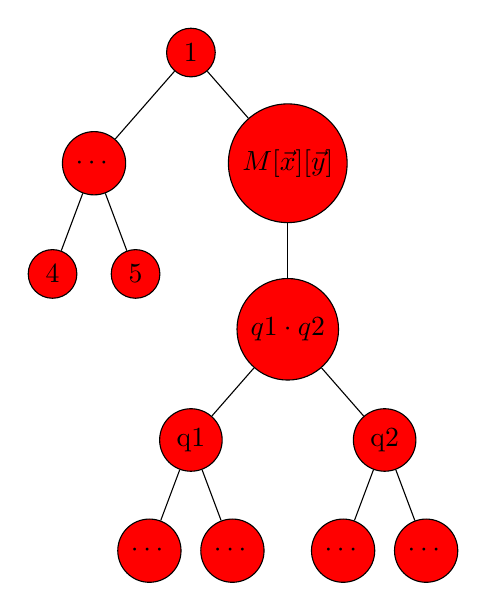
\begin{tikzpicture}%[level/.style={sibling distance=40mm,level distance=15mm}]
[level 1/.style={circle, draw,scale=1.0, fill=red,
    level distance=40pt, sibling distance=70pt},
    level 2/.style={circle, draw, scale=1.0,
    level distance=60pt, sibling distance=70pt},
    level 3/.style={circle, draw, scale=1.0,
    level distance=40pt, sibling distance=70pt},
    level 4/.style={circle, draw, scale=1.0,
    level distance=40pt, sibling distance=30pt}]
    \tikzstyle{every node}=[circle,draw,fill=red]
    \node[] (a){1}
        child { 
            node [](b){$\cdots$}
            child[sibling distance=30pt,level distance=40pt]{
            	node{4}
            }
            child[sibling distance=30pt,level distance=40pt]{
            	node{5}
            }
        }
        child{ 
        		node[](c){$M[\vec{x}][\vec{y}]$}
        		child{
        			node[](d){$q1\cdot q2$}
        			child{
        				node[](f){q1}
        				child{node[](g){$\cdots$}}
        				child{node(h){$\cdots$}}
        				}
        			child{
        				node[](i){q2}
        				child{node[](j){$\cdots$}}
        				child{node(k){$\cdots$}}
        				}
        			}
		};
\end{tikzpicture}
\end{center}
\caption{Tree representation}
\label{fig:map}
\end{figure}

The algorithm starts with node 1, which represents the root of the parse tree. It recursively goes through each of the leaves, therefore constructs the variable vector and also the DBT-domain for each variable.
	
We have mentioned that besides map nodes, there are two more types of intermediate nodes: the union node and the join node. When a union node is met, then it is known that DBT-domains of variables will not pass over this operator and for that the variables and their DBT-domains, which were obtained in the parent, will be passed to each of this node's children. Thus it applies the distribution rule of the join operator over the union operator. For example if we have $ q_{1} * (q_{2} * q_{3} + q_{4} * q_{5}) \equiv q_{1} * q_{2} * q_{3} + q_{1} * q_{4} * q_{5}$, the variables and DBT-domain obtained for $q1$ will be passed both to $q_{2}*q_{3}$ and $q_{3}*q_{4}$, without modifying any of the DBT-domains, regarding that some DBT-domains may change on one branch, for example $q2*q3$. For the other type of node, the join node, the passing of DBT-domains is allowed, and therefore a DBT-domain can be refined by the relation on the right side of the parent node.
	
Every time the algorithm encounters a map then it will create the DBT-domain for that specific map. Here we can make a difference between input and output variables, because the DBT-domain of input variables is dependent on the DBT-domains of output variables from the left side of the map's parent node, and the DBT-domain of the output variables are going to be produced by the children of the map's node. %All this information will be stored in a global variable which can be easily accessed.

A node which is represented by a map will have only one child, because as we mentioned in the definition of the AGCA expression, a map can be defined over an expression or expressions: $M[\vec{x}][\vec{y}]\coloneqq q$
\begin{theorem}
Algorithm \ref{alg1} computes the DBT-domain of each variables and maps.
\end{theorem}

\begin{proof}
The proof is by induction on the height of the tree. The theorem is held for a tree consisting of only one node. Since this node is a simple relation and the Algorithm \ref{alg1} goes  through lines \ref{line10}-\ref{line2}. As we defined, the DBT-domain of any empty set is infinite(all possible values) so the DBT-domain is correctly computed in line \ref{line2}.

Now suppose that the Algorithm \ref{alg1} works for all the trees of a height less than $k$. We want to prove that it will work as well for trees of height $k$. Let $T$ be a tree with height $k$. If root represents a map, it has a child and we correctly computed its output DBT-domain, so the same is held for the map itself and the theorem follows in this case. Otherwise
the root should have two children. The height of both of these children should be less than $k$. So we have correctly compute the DBT-domain of the left child and its input variable. Now we have two cases, if the root node is a union node or a join node. If this is a union node then we can compute the DBT-domain of the right child independently, since no information is passed over the ``+'' in DBToaster\cite{1}. We compute the DBT-domain of the root according to definition \eqref{def:plus}. But if the root node is a join node, we have to pass the information from left child to the right child, since the right child may have some input variables which are defined in the left child. This is done in lines \ref{line:join1},\ref{line:join2}.\par
Thus in either of two cases we compute the DBT-domain of the root correctly and the theorem follows.
\end{proof}
With the above theorem we have the following corollary which helps us in section~\ref{sec:MaintainingDomainswithmultiplicity} for giving some efficient algorithm for maintaining the \dom{}s. 
\begin{corollary}
\label{col:arity0}
The multiplicity order of a tuple in the DBT-domain of a simple relation will always be greater than 0.
\end{corollary}
\section{Defining the multiplicity order of a tuple}

\subsection{Definitions}\label{Multip-def}

Having the definitions for the DBT-domains, we will try to give some insight regarding to the notion of multiplicity order of a tuple. We will start with an example relation: $$q=R(a,b)\cdot S(b,c)$$ the schema for q will have three variables $(a,b,c)$. The multiplicity of a tuple is the number of its occurrences in the relation, in other words the order of multiplicity of that tuple. The multiplicity of a tuple will increase or decrease if insertions or respectively deletions will be made to a relation. For example:
\begin{table}[ht]
\centering
\begin{tabular}{c c c c}
	R & a & b & multip order\\ [0.2ex]
	\hline
	  & $\langle $1 & 2$\rangle$ & 1 \\
	  & $\langle $1 & 3$\rangle$ & 2 \\
	  & $\langle $3 & 4$\rangle$ & 1 \\
\end{tabular}
\caption{Relation $R$}
\end{table}
\begin{table}[ht]
\centering
\begin{tabular}{c c c c}
	S & b & c & multip order\\ [0.2ex]
	%heading
	\hline
	  & $\langle $1 & 1$\rangle$ & 1 \\
	  & $\langle $2 & 2$\rangle$ & 2 \\
	  & $\langle $3 & 5$\rangle$ & 2 \\
\end{tabular}
\caption{Relation $S$}
\end{table}
\begin{table}[ht]
\centering
\begin{tabular}{c c c c c}
	$R\cdot S$ & a & b & c & multip order\\ [0.2ex]
	%heading
	\hline
	  & $\langle $1 & 2 & 2$\rangle$ & 2 \\
	  & $\langle $1 & 3 & 5$\rangle$ & 4 \\
	  & $\langle $3 & 4 & $*\rangle$ & 0 \\
	  & $\langle *$ & 1 & 1$\rangle$ & 0 \\
\end{tabular}
\caption{Relation $R\cdot S$}
\end{table}

We need to maintain the maps for certain values as long as the multiplicity order of a tuple is greater then 0. If the multiplicity order of the tuple drops to 0 then the tuple will not be taken into consideration and therefore it can be eliminated from the DBT-domains of the maps.

We need to store the multiplicity order inside each map and also way to compute the this multiplicity order of an AGCA expression. Since we substitute the subexpressions with maps, we can easily consider the relations as the maps without input variables. Also a map with input variables can be seen as a relation with a group-by clause. Input variable of a map bind some variables. Thus if we compute the map values by all different combinations of these variables, we will look up into these values and return the appropriate value according to the input variables.  

We define the function \emph{arit} which will be used to compute the multiplicity order of a tuple in a certain relation. The function will be defined on the relation and the tuple for which the multiplicity order is desired to be computed. $$arit(\text{Relation } q,\text{Tuple } t)=\text{multiplicity order of }t\text{ in the } q =\pi_{t}(q)$$ where $\pi_{t}(q)$ means the projection of relation $q$ for the tuple $t$. This function can be used for the computation of the multiplicity order of the expressions from the AGCA: $q\coloneqq q\cdot q\text{ }|\text{ }q+q\text{ }|\text{ }q \theta t\text{ }|\text{ }t\gets q\text{ }|\text{ constant}\text{ }|\text{ variable}$. However constants and variables can be eliminated from the computation because relations are of interest.

\begin{align}
arit(q_{1}\cdot q_{2},t)&=\sum\limits_{\{t_{1}\}\Join \{t_{2}\}={t}}^{}arit(q_{1},t_{1})*arit(q_{2},t_{2})\\
arit(q_{1} + q_{2},t)&=arit(q_{1},t)+arit(q_{2},t)\text{, where Schema}(q_{1})\\=\text{Schema}(q_{2})\\
arit(v_1\text{ } \theta \text{ } v_2,t)&=\begin{cases}1,& \mbox{if } v_1\theta v_2 \mbox{ is true and }v_{1}\in t \land v_{2}\in t\\
0,& \text{otherwise} \mbox{ is false} 
\end{cases}\\
arit(v\gets q,t)&=\begin{cases}0, \mbox{ if $t\setminus\{v\}\not\in \text{\dom}_{Schema(t)}(q)$}\\ 1, \mbox{ otherwise} \end{cases}
\end{align}

\subsection{Extending the notion of DBT-domains to multiplicity order}\label{DBT-multip}

In the first part of the document we have talked about the definition of DBT-domains. Now we are going to talk about a combination between DBT-domains of tuples and the multiplicity order of those tuples. We can define something like the following:

$$\multip{}_{\vec x}(R(\vec y))=\bigg\{(\vec c,arit)\Big|\,\sigma_{\forall i:x_i\in\vec{y}\land x_{i}=c_{i}}R(\vec y)= arit \land arit \not= 0\bigg\}$$ 

The notion $\multip{}$ will help us construct both DBT-domains for each variable, but also compute the correct order of multiplicity of a tuple within a relation. If we have, for example, a relation $R$ with the following schema $R(\vec y=\langle x_1,x_2,\cdots,x_n\rangle)$ and know that only a part of the variables defined by the schema are used for data flow to other relation $\vec x=\langle x_i,x_{(i+1)},\cdots,x_{(i+j)}\rangle$, then the $\multip{}_{\vec x}(R(\vec y))$ will be all the groups of unique tuples with their order of multiplicity. This would be the same with having a query on relation $R$ with a group by using $\vec x$:
$$\mbox{SELECT }\vec{x} \mbox{,COUNT(*) FROM }R \mbox{ GROUP BY }\vec{x}$$
The query will produce a table with all the tuples and their multiplicity order. The tuples will be unique.

For example:

\begin{table}[H]
\centering
\begin{tabular}{c c c c c}
	R & a & b & c & d\\ [0.2ex]
	%heading
	\hline
	  & $\langle $1 & 2 & 4& 3$\rangle$\\
	  & $\langle $2 & 3 & 5 & 4$\rangle$\\
	  & $\langle $7 & 2 & 5 & 2$\rangle$\\
	  & $\langle $6 & 3 & 9 & 4$\rangle$\\
	  & $\langle $11 & 2 & 4 & 2$\rangle$\\
	  & $\langle $1 & 2 & 9 & 3$\rangle$\\
	  & $\langle $3 & 3 & 5 & 5$\rangle$\\
	  & $\langle $3 & 2 & 5 & 2$\rangle$\\
	  & $\langle $3 & 2 & 5 & 3$\rangle$\\
\end{tabular}
\caption{Relation $R$}
\end{table}

In table 1 we have the relation $R$ with the schema $\vec y=\langle a,b,c,d\rangle$. From that schema there are being used only two variables, $\vec x=\langle b,d\rangle$ for the communication with other relation from a specific query. Applying the query presented in the previous paragraph we can compute all the unique tuples of $\vec x$ and their multiplicity order.

\begin{table}[H]
\centering
\begin{tabular}{c c c c}
	$\multip{}_{\langle b,d\rangle}(R)$ & b & d & arit \\ [0.2ex]
	%heading
	\hline
	  & $\langle $2 & 3$\rangle$ & 3\\
	  & $\langle $3 & 4$\rangle$ & 2\\
	  & $\langle $2 & 2$\rangle$ & 3\\
	  & $\langle $3 & 5$\rangle$ & 1\\
\end{tabular}
\caption{Relation $R$}
\end{table}

Taking into account the rule defined for the computation of the $\multip{}$, we are going to have for relation $R$ the following:
$$\multip{}_{\langle b,d\rangle}(R(\langle a,b,c,d\rangle))=\{((2,3),3),((3,4),2),((2,2),3),((3,5),1)\}$$

So far we have explained only one type of expression in the AGCA: the simple relation $R(\vec y)$, however AGCA presents many more types. Therefore we have to explain each of other types of expression. We remind that in AGCA an expression q may be of the following form:
\begin{equation}
q\coloneqq q\cdot q | q + q|v \gets q |v_{1}\theta v_{2}|R(\vec{y})|\text{c}|\text{v}|(M[\vec{x}][\vec{y}]:-q)
\end{equation}
Exactly as we did with the definitions for the DBT-domains, we can write the definitions for the DBT-domains with multiplicity order just extending the definition of the DBT-domain. For $q\coloneqq v_{1}\theta v_{2}$:
\begin{align}
\text{\multip{}}_{\vec{x}}(v_{1}\theta v_{2})=\bigg\{(\vec{c},arit)\,\Big|\,\forall i,j:\nonumber\\(v_{1}=x_{i}\land v_{2}=x_{j})\Rightarrow (c_{i}\theta c_{j}=arit)\bigg\}
\end{align}
For $q\coloneqq q_{1}\cdot q_{2}$:
\begin{align} 
\text{\multip}_{\vec{x}}(q_{1}\cdot q_{2})=\big\{(\vec{c},arit)\,\big|(\vec{c},arit_{1})\in&\text{\multip}_{\vec{x}}(q_{1})\nonumber\\\land (\vec{c},arit_{2})\in\text{\multip{}}_{\vec{x}}(q_{2})& \land arit= arit_{1}\times arit_{2}\big\}
\end{align}
For $q\coloneqq q_{1}+q_{2}$:
\begin{align}
\text{\multip{}}_{\vec{x}}(q_{1}+ q_{2})=&\{(\vec{c},arit)\,|((\vec{c},arit_{1})\in\text{\multip{}}_{\vec{x}}(q_{1})\nonumber\\&\lor(\vec{c},arit_{2})\in\text{\multip{}}_{\vec{x}}(q_{2}))\nonumber\\&\land arit=arit_{1}+arit_{2}\}
\end{align}
For $q\coloneqq t\gets q$:
\begin{align}
\text{\multip{}}_{\vec{x}}(v\gets q)=\Big\{(\vec{c},arit)\Big|\vec{c}\in\text{\dom{}}_{\vec{x}}(q)\land \bigg(\Big(\big(\forall i: (x_{i}=v) & \nonumber\\\Rightarrow(c_{i}=q)\big)\land (arit=1)\Big)\lor (arit=0)\bigg)\Big\}
\end{align}

\section{Multiplicity order computation}

We have defined some rules for the computation of the DBT-domains and the multiplicity order of each tuple within a DBT-domain. Having them, we can start writing an algorithm to compute the DBT-domains and the tuples' multiplicity order. We will start with the algorithm that will compute the DBT-domains and multiplicity order for each element. The algorithm will be similar to the algorithm that we have written for determining only the DBT-domains of variables that appear within a query.

As the algorithm presented for the computation of the DBT-domains, this one must have as well a structure which will help in the computation.

\begin{program}
\begin{alltt}
struct \{
x: the vector of all the variables 
DBT-multip: the DBT-domain and multiplicity order of all the variables
\}
\end{alltt}
\caption{$nodeMultipOrderAttribute$}
\label{struct1}
\end{program}

Algorithm~\ref{alg3} is similar to the Algorithm~\ref{alg1}. The steps are the same, we traverse the parse tree, seeking all the nodes and test them to find out the type. The basic mechanism is the same when talking about reaching a node that will be a union node or a join node or even a map node. The difference will appear at the results presented, because in  Algorithm~\ref{alg1} we will compute only DBT-domains of each tuple, whilst in Algorithm~\ref{alg3} we will compute the combination between the DBT-domains and the multiplicity order of each tuple inside the DBT-domains.

Instead of using the definitions that we have written in Section~\ref{sec:definingdomains}, we will use the definitions presented in Subsection~\ref{DBT-multip}. These definitions are just an extension of the definitions from the DBT-domains, however they will also make use of the functions for computing the multiplicity order presented in Subsection~\ref{Multip-def}.

The rules for join expressions and union expression will remain the same. In the case of join expressions we will take only the common tuples, and in the case for union expressions we will take all the tuples. The difference here will be that for each tuple we will have the multiplicity order. As shown in Subsection~\ref{Multip-def}, if we have join expressions then a tuple that is common to those expression will have the multiplicity order equal with the product of the multiplicity orders from the two expression. If we have a union expression, the tuples will maintain their multiplicity order only if the tuples are not common. If the tuples are common between $q_1$ and $q_2$ the multiplicity order of the tuple will be the sum of them.

\begin{algorithm}[H]
\caption{computeMultipOrder($node$,$s$)} 
\label{alg3}
\textbf{Input:} $node$ as the root of the tree to be traversed, and $s$ which is of type $nodeMultipOrderAttribute$ \\
\textbf{Output:}  $result$ of type $nodeMultipOrderAttribute$ that contains vector of variables $\vec x$ and the DBT-domains of each variable with multiplicity order
\begin{algorithmic}[1]
\IF{$node.type=$``+''}
\STATE  $s_{1}\gets$ computeMultipOrder($node.left, s$)
\STATE  $s_{2}\gets$ computeMultipOrder($node.right, s$)
\STATE  $result.\vec{x}\gets s_{1}.\vec{x} \cup s_{2}.\vec{x}$
\STATE  $result.\multip{}\gets \{(\vec{c},arit)|(\vec{c_{1}},arit_{1})\in s_{1}.\multip{}\land (\vec{c_{2}},arit_{2})\in s_{2}.\multip{}\land (\vec{c_{1}}=\vec{c_{2}}\Rightarrow (\vec{c},arit)=(\vec{c_{1}},arit_{1}+arit_{2}))\land (\vec{c_{1}}\not=\vec{c_{2}}\Rightarrow (\vec{c},arit)=(\vec{c_{1}},arit_{1})\lor (\vec{c},arit)=(\vec{c_{2}},arit_{2}) )\}$
\ELSIF{$node.type=$``*''}\label{join:statement}
\STATE  $s_{1} \gets \text{computeMultipOrder}(node.left, s)$
\STATE $result\gets \text{computeMultipOrder}(node.right, s_{1})$
\ELSIF{$node.type=$``Map''}
\STATE $node.\vec{x}\gets s.\multip{}$
\STATE $s_{1}\gets\text{computeMultipOrder}(node.child,s)$
\STATE $node.\vec{y}\gets s_{1}.\multip{}$
\STATE $result.\vec{x}\gets s_{1}.\vec{x}$
\STATE $result.\multip{}\gets node.\vec{y}$
\ELSE 
\STATE $result.\vec{x}\gets s.\vec{x} \cup \{\text{Var$(node)$}\}$
\STATE $aux \gets extendMultipOrderToSchema_{result.\vec{x}}(s.\multip{})$
\STATE $result.\multip{}\gets \{(\vec{c},arit)|(\vec{c},arit_{1})\in aux\land (\vec{c},arit_{2})\in \multip{}_{result.\vec{x}}(node) \land (arit=arit_{1}*arit_{2}) \}$
\ENDIF
\RETURN $result$
\end{algorithmic}
\end{algorithm}

\section{Maintaining the DBT-domains using the multiplicity order of a tuple}
\label{sec:MaintainingDomainswithmultiplicity}
The main goal is to maintain the DBT-domains of the variables of each map that are presented in query expression. We give a solution of maintaining these DBT-domains, see how the DBT-domains will increase or decrease if tuples are being added or deleted from the relations.
\subsection{Algorithm 1}

The algorithm traverses the parse tree until it reaches the leaf that represents the relation that needs an update. Therefore a Depth First Algorithm can be used. First we shall talk about inserting a new tuple to an existing relation. When a leaf with the specified relation is encountered, we check if the tuple already exists in the set of multiplicity order. If the tuple exists, then we will retrieve the multiplicity order, and just for the fact that it exists in the DBT-domain of a relation the multiplicity order of a tuple will be greater than 0. We increment the multiplicity order and repack everything and put it back in the set. If the tuple is not found in the DBT-domain of the relation that means that we will have a transition of the multiplicity order from $0 \rightarrow 1$, because we have to add the tuple to the existing DBT-domain, and therefore we have to recompute the DBT-domains for each and every map starting from that leaf.

When talking about making a deletion of a tuple inside a relation, most of the algorithm will remain the same. We should first find the leaf that represents the designated relation, find if the tuple is or is not inside the DBT-domain of the relation. If the tuple is not inside the DBT-domain then there appears an error because you can not delete something from the table of database without that tuple appearing inside the table. Therefore the tuple that is going to be deleted must appear in the DBT-domain of the relation. Having the group (\dom{},\multip) we can test the multiplicity order. If the multiplicity order, after deleting the tuple, remains greater than 0 then the algorithm stops by making the modification to the multiplicity order, packing the results and putting it back into the set of the DBT-domain. Otherwise, if the multiplicity order drops to 0, then we will have a transition of $1 \rightarrow 0$ and thus we have to recompute each and every DBT-domain of the maps starting from the leaf that suffered a change.
To conclude the small description of the algorithm, we are interested only in transitions $0 \rightarrow 1$ or $1 \rightarrow 0$, because only then we will have to recompute every DBT-domain of the maps.

A sketch of the algorithm would look like as follows:

\begin{algorithm}[H]
\caption{$maintain_{DBTdomains}$($node$,$tuple$,$R$,$op$)} 
\label{alg2}
\textbf{Input:} $node$ - root of parse tree, $tuple$ - the new tuple, $R$ - name of the relation, $op$ - operation: add or delete \\
\textbf{Output:} it returns a list of tuples with their appropriate multiplicity order\\
\begin{algorithmic}[1]
\IF{$node.type=$``Map''}
\STATE $list\gets maintain_{DBTdomains}(node.child,tuple,R,op)$
\IF{$list\not=NULL$}
\FORALL{$elem\in list$}
\STATE $(list_{new},node)=updateNode(elem,node,op)$
\ENDFOR
\RETURN  $list_{new}$
\ENDIF
\RETURN  $NULL$
\ELSIF{$node.type=$''Relation''}
\IF{the name of the relation is $R$}
\RETURN  $\{(tuple,op)\}$
\ENDIF
\RETURN $NULL$
\ELSIF{$node.type\neq$``$\theta$'' \AND $node.type\neq$``$\gets$''}
\STATE $s_{1}\gets maintain_{DBTdomains}(node.left,tuple,R,op)$
\STATE $s_{2}\gets maintain_{DBTdomains}(node.right,tuple,R,op)$
\IF{$op=1$}
\IF{$node.type=$''*''}
\STATE $s_{1}\gets computeCommon(s_{1},node.right)$
\STATE $s_{2}\gets computeCommon(s_{2},node.left)$
\ENDIF
\ELSIF{$node.type=$''+''}
\STATE $s_{1}\gets computeDifference(s_{1},node.right)$
\STATE $s_{2}\gets computeDifference(s_{2},node.left)$
\ENDIF
\RETURN  $s_{1}\cup s_{2}$
\ENDIF
\RETURN $NULL$
\end{algorithmic}
\end{algorithm}

\begin{algorithm}[H]
\caption{computeCommon($list$,$node_{map}$)}
\label{alg4}
\textbf{Input:} $list$ - a list of tuples with their multiplicity order, $node_{map}$ - as the node map\\
\textbf{Output:} a list of common tuples from the $node_{map}$\\
\begin{algorithmic}[1]
\STATE $s\gets NULL$
\IF{$list\not=NULL$}
\FORALL{$elem\in list$}
\IF{$(elem\in node.\vec{y})\lor(elem\in node.\vec{x})$}
\STATE recompute multiplicity order of $elem.tuple$
\STATE $s\gets s \cup elem$
\ENDIF
\ENDFOR
\ENDIF
\RETURN  $s$
\end{algorithmic}
\end{algorithm}

\begin{algorithm}[H]
\caption{computeDifference($list$,$node_{map}$)}
\label{alg5}
\textbf{Input:} $list$ - a list of tuples with their multiplicity order, $node_{map}$ - as the node map\\
\textbf{Output:} a list of common tuples from the $node_{map}$\\
\begin{algorithmic}[1]
\STATE $s\gets NULL$
\IF{$list\not=NULL$}
\FORALL{$elem\in list$}
\IF{$(elem\notin node.\vec{y})\land(elem\notin node.\vec{x})$}
\STATE $s\gets s \cup elem$
\ENDIF
\ENDFOR
\ENDIF
\RETURN $s$
\end{algorithmic}
\end{algorithm}

\begin{algorithm}[H]
\caption{updateNode($elem$,$node$,$op$)}
\label{alg6}
\textbf{Input:} $elem$ - the tuple that needs to be checked,$node$ - the map node, $op$ - operation\\
\textbf{Output:} (list of tuples,the new domain)\\
\begin{algorithmic}[1]
\IF{op=1}
\IF{$elem\notin node.\vec{y}$}
\STATE $node.\vec{y}\gets node.\vec{y} \cup elem$
\STATE $list_{new}\gets list_{new}\cup elem$
\ENDIF
\ELSE
\IF{$elem\in node.\vec{y}$}
\STATE $update(node.\vec{y},elem)$
\IF{elem.ord=0} 
\STATE delete it from $node.\vec{y}$
\STATE $list_{new}\gets list_{new}\cup elem$
\ENDIF
\ENDIF
\ENDIF
\RETURN ($list_{new}$,$node$)
\end{algorithmic}
\end{algorithm}\textbf{}

Algorithm~\ref{alg2} maintains the domains of each map. It traverses the tree structure that we have introduced in Section~\ref{DBT-domain}. For each expression it computes the tuples that are being produced due to an insertion/deletion in to/from a specified relation.

We will have two cases:
\begin{enumerate}
\item adding a tuple to a relation($op=1$)

When adding a tuple to a relation we have to see if the tuple is in the \dom{} of that relation or not. If it is we do not make any changes. Otherwise, we have to make the necessary changes to the \dom{} of the relation. We produce a list of tuples that were modified by the added tuple and pass it to the higher expressions.

When we have union expressions like $q_1+q_2$, all the tuples produced by the insertion, both from $q_1$ and $q_2$, will be taken to the \dom{} of the union expression. However in join expressions like $q_1\cdot q_2$, we take only the common tuples between the two expressions, therefore using the function~\ref{alg4}, which will compute only those tuples that are common, and of course will also compute the new multiplicity order of those tuples.
\item deleting a tuple from a relation($op=-1$)

When deleting a tuple from a relation, we need to know if the multiplicity order of the specific tuple changes in the \dom{}. If the multiplicity order drops to zero, this will mean that the tuple is not anymore in the relation and therefore it will need to be deleted. We create a list with those tuples that have the multiplicity order equal with 0 and pass the list to the higher expression.

When we have join expressions $q_1\cdot q_2$, the deletion will be without any kind of problems. If a tuple disappears from one expression $q_1$ or $q_2$, it will disappear from $q_1\cdot q_2$, because the tuple won't be any more a common tuple. A difficulty appears when talking about union expressions $q_1+q_2$. If we will delete a tuple from $q_1$, that does not mean that the tuple will be deleted from the union expression. If the deleted tuple from $q_1$ also appears in the \dom{} of $q_2$, then the tuple won't be deleted from $q_1+q_2$, only the order of multiplicity changes. Therefore, we have to compute the difference between the list of tuples produced from an expression and the \dom{} of the other expression. This is done by the function~\ref{alg5}.
\end{enumerate}

The function~\ref{alg6} helps us in refreshing the \dom{}s of each node and produces the list of tuples that needs to be passed to the higher expression for their update as well. When adding a tuple, we test only if the tuple that was added is not in the \dom{}, and only then we add it to the list. When deleting a tuple, the tuple must be in the \dom{}, therefore the multiplicity order will change, and we have to test only if that multiplicity order has dropped to 0. Only then we add the tuple to the list.

\subsection{Algorithm 2}
In this section we give an algorithm for computing the DBT-domains incrementally after each deletion or insertion. Let $T$ be the parse tree as we had in the previous sections. We want to know how the DBT-domain of each node changes with any insertion or deletion from any relations. If the DBT-domain of any leaves of $T$ changes, in the worst case we need to re-evaluate DBT-domains of all the nodes in $T$. For an example, suppose the leftmost leaf changes and all other leaves depends on it, like $R(\vec{y})\cdot\prod_{i}{(y_{i}>a_{i})}$ where $a_{i}$ are constants.
Although in the worst case we need to reevaluate the DBT-domains of all nodes, but in some cases we can have some optimization in order to avoid recomputing the DBT-domains. We define function \InputVars{} to a function that takes a node and returns its input variables. We can define a similar function \OutputVars{} for output variables.
\begin{align}
\text{\InputVars}(R(\vec{y}))&=\{\}\\
\text{\InputVars}(v_{1}\theta v_{2})&=\{v_{1},v_{2}\}\\
\text{\InputVars}(q_{1}+q_{2})&=\text{\InputVars}(q_{1})\cup\text{\InputVars}(q_{2})\\
\text{\InputVars}(q_{1}\cdot q_{2})&=\text{\InputVars}(q_{1})\cup\text{\InputVars}(q_{2})-\text{\OutputVars}(q_{1})\\
\text{\InputVars}(v\gets q_{1})&=\text{\InputVars}(q_{1})\\
\text{\OutputVars}(R(\vec{y}))&=\vec{y}\\
\text{\OutputVars}(v_{1}\theta v_{2})&=\{\}\\
\text{\OutputVars}(q_{1}+q_{2})&=\text{\OutputVars}(q_{1})\cap\text{\OutputVars}(q_{2})\\
\text{\OutputVars}(q_{1}\cdot q_{2})&=\text{\OutputVars}(q_{1})\cup\text{\OutputVars}(q_{2})\\
\text{\OutputVars}(v\gets q_{1})&=\{v\}
\end{align}
According to the above definitions we can give an algorithm for computing the changes to each map for any insertion or deletion to/from any relation. For our purpose we need a way to show the set of relations contains in each node, we show this by \Rel{} and define it as follow:
\begin{align}
\text{\Rel}(R(\vec{y}))&=R\\
\text{\Rel}(v_{1}\theta v_{2})&=\{\}\\
\text{\Rel}(q_{1}+q_{2})&=\text{\Rel}(q_{1})\cup\text{\Rel}(q_{2})\\
\text{\Rel}(q_{1}\cdot q_{2})&=\text{\Rel}(q_{1})\cup\text{\Rel}(q_{2})\\
\text{\Rel}(v\gets q_{1})&=\text{\Rel}(q_{1})
\end{align}

\begin{algorithm}
\caption{CheckRightNode($node,v_{1},R,s$)}
\label{alg:sub}
\textbf{Input:} $node$ as the root of the tree to be traversed, $v_{1}$ a flag indicating if the left subtree has changed, $R$ the relation to be modified and $s$ as the structure \\
\textbf{Output:} A pair whose first element is a boolean to indicate if any DBT-domains in the subtree rooted at $node.right$ has changed
and the second element is the \dom($node.right$)
\begin{algorithmic}[1]
\IF{$R\in$\Rel($node.right$) \OR $(v_{1}=\TRUE\,  \AND\, s.x \,\cap\, $\InputVars $(node.right)\neq\emptyset$ )}
\RETURN MaintainDBT-domains$(node.right,R,s,v_{1})$
\ELSE
\RETURN (\FALSE$,node.right.s)$
\ENDIF
\end{algorithmic}
\end{algorithm}
\begin{algorithm}
\caption{MaintainDBT-domains$(node,R,s,m)$}
\label{alg:MD}
\textbf{Input:} $node$ as the root of the tree to be traversed, $R$ the relation to be modified, $s$ as the structure and $m$ as a modification flag\\
\textbf{Output:} A pair whose first element is a boolean to indicate if any DBT-domains in the subtree rooted at $node$ has changed
and the second element is the \dom($node$)
\begin{algorithmic}[1]
\IF{$R\in$\Rel(node.left) \OR \InputVars(node.left)$\cap s.x\neq\emptyset$ \AND $m=\TRUE$}
\label{lst:ml1}
\STATE $(v_{1},s_{1})\gets \text{MaintainDBT-domains($node.left,R,s,m$)}$
\ELSE
\STATE $(v_{1},s_{1})\gets (\FALSE,node.left.s)$
\ENDIF
\label{lst:ml2}
\IF{$node.type=$``+''}
\STATE $(v_{2},s_{2})\gets$CheckRightNode$(node,v_{1},s)$
\STATE  $node.s.dom\gets \text{\dom}_{node.s.\vec x}(s_{1}.dom)\cup\text{\dom}_{node.s.\vec x}(s_{2}.dom)$
\ELSIF{$node.type=$``*''}
\STATE $(v_{2},node.s.dom)\gets$CheckRightNode$(node,v_{1}\lor m,s_{1})$
\ELSIF{$node.type=$``Relation''}
\STATE Apply changes to the relation if it is $R(\vec{y})$ and set $v_{2}$ \TRUE{} if the DBT-domain changed
\STATE $node.s.dom\gets\text{\dom}_{node.s.\vec{x}}(node)$
\ELSIF{$node.type=$``Map''}
%\label{lst:map}
\STATE $node.\vec{x}\gets\text{\dom}_{s.\vec{x}}(s.dom)$
\STATE $(v_{2},node.\vec{y})\gets$MaintainDBT-domains$(node.child,R,s,m)$%\label{lst:child}
\STATE $result.\vec{x}\gets s.\vec{x}$
\STATE $result.dom\gets node.\vec{y}$
\ELSE
\STATE $node.s.dom\gets \text{\dom}_{node.s.\vec{x}}(s.dom)\cap\text{\dom}_{node.s.\vec{x}}(node)$%\label{line2}
\STATE $v_{2}\gets \FALSE$
\ENDIF
\RETURN $(v_{1}\lor\,v_{2}\lor m,result)$
\end{algorithmic}
\end{algorithm}
As a consequence of Corollary~\ref{col:arity0}, we need to run Algorithm~\ref{alg:MD} if and only if the modification to relation $R$ makes a transition from 0 to 1(for insertion) or from 1 to 0(for deletion). \par 
 The intuition of Algorithm~\ref{alg:MD} is simple. Suppose we want to modify relation $R$ (insertion or deletion).
In each node we have compute the domain of the left child in two cases. First if the left subtree of the node contains $R$, in the other words $R\in$\Rel(node.left), Or the left subtree has some input variables whose domains are changed already during the execution of the algorithm. If so, we continue recursively in the left subtree(lines \ref{lst:ml1}-\ref{lst:ml2}). We run the algorithm on the right subtree if and only if it contains $R$ or some domains have changed due to the modification and the right subtree has some input variables which depend on them. Deciding whether or not to run the algorithm on the right subtree is preformed by Algorithm~\ref{alg:sub}.
According to the type of nodes, as we had in Algorithm~\ref{alg1}, we compute the \dom{} of $node$. Here we suppose that each node has a left and right child as before and structure $s$ as defined in \ref{struct}. We suppose that before any executions of Algorithm~\ref{lst:ml2}, Algorithm~\ref{alg1} has been executed at least one time to initialize . So for each $node$ we have associated a structure $s$. Thus with $s$ we can access to the \dom($dom$) of each node and the set of its variables($\vec{x}$). 

\section{Initial value of maps}
So far we have talked about how the domain will change when you add a new tuple to a relation that appears within a query. Now we try to see how a map will be initialized when adding a tuple to a relation. From $\cite{1}$ we know that the compilation algorithm takes an aggregate query and defines a map for it, which represents the materialized view of the query. The algorithm creates a trigger for each possible update on an event, which will specify how to update the main query. To this operation, the algorithm computes the delta query, and creates a new map that will represent the materialized view of the delta. For example, if we have the following query q:
\begin{equation}
\mbox{SELECT sum(}a\cdot c\mbox{) FROM R(a,b), S(b,c) WHERE } R.b=S.b
\end{equation}
The compilation algorithm takes this query, replaces it with a map $q[][]$, and computes its deltas. We will have two events: $onR$, $onS$. For simplicity we take for now only the inserting operation. The trigger code will look as follows:
\begin{align*}
+onR(a,b)&:\\
&q[][]+=a*m_R[][b]\\
&m_S[][b]+=a\\
\end{align*}\vspace{-40pt}
\begin{align*}
+onS&(b,c):\\
&q[][]+=c*m_S[][b]\\
&m_R[][b]+=c\\
\end{align*}
In \cite{1} a map is defined by as function which takes input values and produces output values. With this definition, we can consider the initialization as a process of computing the function's output values for some new input values without computing the function body.

\section{Equijoins}

We start talking about map initialization in the simplest of cases: queries represented by relations that are joined only by equalities.
\begin{align}
\mbox{SELECT sum(}\cdots\mbox{) FROM }&R_1,R_2,\cdots,R_n\mbox{ WHERE }R_i.x_{ik}=R_j.x_{jt} \label{query1}\\
&(\forall i,j\in\{1..n\}\land i\not=j\land (x_{ik}\in Sch(R_i))\nonumber\\
&\land(x_{jt}\in Sch(R_j))\nonumber
\end{align}

When having only equality joins, the maps defined over expressions consisting of simple relations will have only output variables. Every variable will be bounded to the relations and therefore their \dom{}s will depend on the values provided by these relations.

For query \eqref{query1}, the compilation algorithm will replace it with a map $q[][]$. When computing the delta regarding to a relation $R_k$, $\Delta_{R_k}$, we have a map assigned to the delta. $m_{R_k}[][x_i,\cdots,x_j]$, where $x_i,\cdots,x_j$ are exactly as mentioned up, the variables that have to be replaced by values when an event $onR_k$ will appear. The map can easily be compared with a query, which is simpler and also have a group by clause.

\begin{align}
\text{SELECT}\cdots&\text{ FROM }R_1,R_2,\cdots,R_{k-1},R_{k+1},\cdots,R_n\label{querygen}\\
&\text{ WHERE }R_l.x_{lt}=R_m.x_{ms}\nonumber\\
&(\forall l,m\in\{1\cdots n\}-\{k\}\land l\not=m)\nonumber\\
&\text{GROUP BY } x_i,\cdots,x_j\nonumber
\end{align}
	
Relation $R_k$ have the following schema: $Sch(R_k)={x_1,x_2,x_3,\cdots,x_n}$, but only some variables are going to be used for the communication with the other relations: $x_i,\cdots,x_j$. We  have the trigger $+onR_k(x_1,\cdots,x_n)$, and when such an event appears we  test if the variables $x_i,\cdots,x_j$ from the arguments of $+onR$ are in the \dom{} of the map or not. 
	
We assume that the tuple is not in the \dom{} of the map $m_{R_k}$ and the initial value for the map regarding to that tuple will be different from 0.
$$m_{R_k}[][x_i,\cdots,x_j]\not= 0$$
If this is true then the query that can be generated for the map $m_{R_k}$, exactly like \eqref{querygen}, produce a table, that have a record with the specified tuple, therefore the tuple is in the \dom{} of the map, $\{x_i,\cdots,x_j\in \dom(m_{R_k}) \}$. This contradicts the sentence we assumed at first. Furthermore, when invoking the query for the given values the result of the query will not be $NULL$, and therefore contradicting the fact the that tuple is not defined in the table and the query result should be $NULL$. And therefore any time, a new tuple that is not in the \dom{} only provoke a zero initialization of the map for that tuple.

Taking into account the definitions of the AGCA expressions in \eqref{def:agca}, the following theorem works with a subset of those definitions, namely with:
$$q\coloneqq q\cdot q | q + q|R(\vec{y})|(M[\vec{x}][\vec{y}]\text{::-}q)$$
	
Relation $R_k$ has the following schema: $Sch(R_k)={x_1,x_2,x_3,\cdots,x_n}$, but only some variables are going to be used for the communication with the other relations: $x_i,\cdots,x_j$. We have the trigger $+onR_k(x_1,\cdots,x_n)$, and when such an event appears we will test if the variables $x_i,\cdots,x_j$ from the arguments of $+onR$ are in the \dom{} of the map or not. 
	
We assume that the tuple is not in the \dom{} of the map $m_{R_k}$ and the initial value for the map regarding to that tuple will be different from 0.
$$m_{R_k}[][x_i,\cdots,x_j]\not= 0$$
If this is true then the query that can be generated for the map $m_{R_k}$:
\begin{align*}
\mbox{SELECT}\cdots&\mbox{ FROM }R_1,R_2,\cdots,R_{k-1},R_{k+1},\cdots,R_n\\
&\mbox{ WHERE }R_l.a=R_m.a\\
&(\forall l,m\in\{1\cdots n\}-\{k\}\land l\not=m)\\
&\mbox{GROUP BY } x_i,\cdots,x_j
\end{align*}
 produces a table, that has a record with the specified tuple, therefore the tuple will be in the \dom{} of the map, $\{x_i,\cdots,x_j\in \dom(m_{R_k}) \}$. This contradicts the sentence we assumed at first. 
 %Furthermore, when invoking the query for the given values the result of the query will not be $NULL$, and therefore contradicting the fact the that tuple is not defined in the table and the query result should be $NULL$. And therefore any time, a new tuple that is not in the \dom{} will only provoke a zero initialization of the map for that tuple.

\begin{theorem}
\label{thm:1}
The value of a map for a specific tuple, which is not in the \dom{} of the map, will always be 0.
\end{theorem}
$$\vec{y}\notin\dom{}_{\vec{x}}(q)\Rightarrow m_q[][\vec{y}]=0$$

\begin{proof}
We will give a proof based on induction on the parse tree.

We presume that the map is defined over a simple relation: $m_R[][\vec{y}]\coloneqq R(\vec{y})$. The vector $\vec{y}$ from the output variables of the maps will correspond to the $\vec{y}$ from the simple relation. Therefore the following statement is true: $\dom{}_{\vec{x}}(m_R[][\vec{y}])=\dom{}_{\vec{x}}(R(\vec{y}))$.

If we add tuple $\vec{y_1}=\langle y_1,y_2,\cdots,y_n\rangle$ to the relation $R$, we are going to have two situations:
\begin{enumerate}
\item $\vec{y_1}\in\dom{}_{\vec{x}}(R(\vec{y}))$, therefore the \dom{} of the relation remains the same and the map is already instantiated.
\item $\vec{y_1}\notin\dom{}_{\vec{x}}(R(\vec{y}))$. If the tuple is not in the \dom{}, then $$\dom{}_{\vec x}(R(\vec y))\cup=\vec{y_1}\mbox{ and }m_{R}[][\vec{y_1}]=0$$ because the order of multiplicity of that tuple in $R$ was zero and thus any operation (sum, count) produces a NULL result.
\end{enumerate}
Therefore, $\vec{y_1}\notin\dom{}_{\vec{x}}(R(\vec{y}))\Rightarrow m_R[][\vec{y_1}]=0$ and the base case is true.

First we talk about join relations and maps defined over a join of expressions: $m_q[][\vec{y}]:=q_1\cdot q_2$. Definition \ref{def:join} says that the \dom{} of a join expression is the intersection between the \dom{}s of $q_1$ and $q_2$. If $\vec{y_1}\notin\dom{}_{\vec{x}}(q_1\cdot q_2)$ then we will have the following cases:
\begin{enumerate}
\item $\vec{y_1}\notin\dom{}_{\vec{x}}(q_1)$ which means that the map defined over the relation $q_1$ will be 0 for that tuple.
\begin{equation}
\Big(\big((\llbracket q_{1}\rrbracket(\cdot)=0)\land (q\coloneqq q_{1}*q_{2})\big)\Rightarrow (\llbracket q\rrbracket(\cdot)=0)\Big)\Rightarrow m_{q}[][\vec{y_{1}}]=0
%m_{q_1}[][\vec{y_1}]=0\land m_q[][\vec{y_1}]: m_{q_1}[][\vec{y_1}]*m_{q_2}[][\vec{y_1}]\Rightarrow m_{q}[][\vec{y_1}]=0*m_{q_2}[][\vec{y_1}]=0
\end{equation}
%where $m_{q_1}[][\vec{y_1}]::q_1$ and $m_{q_2}[][\vec{y_1}]::q_2$.
\item $\vec{y_{1}}\notin\dom{}_{\vec{x}}(q_2)$ the same proof as in the first case, but now for the expression $q_2$.
\end{enumerate}

Secondly we consider union expressions and maps defined over union expressions: $m_q[][\vec{y}]::q_1+q_2$. Definition \ref{def:plus} says that the \dom{} of a union expression is the union between the \dom{}s of $q_1$ and $q_2$. Therefore, if $\vec{y_{1}}\notin\dom{}_{\vec{x}}(q_1+q_2)$ then: $\vec{y_{1}}\notin\dom{}_{\vec{x}}(q_1)\land \vec{y_{1}}\notin\dom{}_{\vec{x}}(q_2)$.
\begin{equation}
\Big(\big((\llbracket q_{1}\rrbracket(\cdot)=0)\land (\llbracket q_{2}\rrbracket(\cdot)=0)\land(q\coloneqq q_{1}+q_{2})\big)\Rightarrow (\llbracket q\rrbracket(\cdot)=0)\Big)\Rightarrow m_{q}[][\vec{y_{1}}]=0
\end{equation}
%where $m_{q_1}[][\vec{y_1}]::q_1$ and $m_{q_2}[][\vec{y_1}]::q_2$.
\end{proof}
As the result of Theorem~\ref{thm:1}, we can consider Algorithm Compile in \cite{1}. Algorithm Compile uses the initial value of map $t$ as $t_{init}$. As a consequence of Theorem~\ref{thm:1}, we can say that whenever $t$ consists of only equal joins we know that the $t_{init}$ is always zero, otherwise we need to compute it as before.\\ \par
Another problem of initial value computation, besides the problem of with which value should a map be initialized, is the problem of how fast to do the initialization. We have two different sorts of initializations: an eager one and a lazy one. The eager one initializes the right side of a trigger expression, when the left side of the expression is initialized. The right side is initialized if and only if it needs initialization. And the lazy one is based on the fact that only the left side will be initialized, and the right side no, leaving the rest side of the initialization to be done when the appropriate trigger is called.

\subsection{Map initialization}

We have talked in section~\ref{sec:definingdomains} about maps as being total function. The definition says that a total function is a function that has a value for each variable in the domain on which the function is defined. In this subsection we want to talk about when to initialize a map and how this is connected with the completion of maps offered by DBToaster.

For example, if we have the following trigger code:

\begin{align}
\label{example}
&+onS(b,c):\\\nonumber
&q[][]+=m_{S_1}[][b]*m_{S_2}[][c]\\\nonumber
&m_R[][b]+=m_{RS}[][c]\\\nonumber
&m_{RT}[][b,c]+=1\\\nonumber
\end{align}

When talking about map initialization we can have to situations:
\begin{enumerate}
\item initialize the left and the right side of the expression when adding a new tuple to a relation

In example~\ref{example} we have $m_R[][b]+=m_{RS}[][c]$. When we add a new tuple $\langle b,c\rangle$ to relation $S$ we initialize both map $m_R[][b]$ and $m_{RS}[][c]$ with the appropriate value

\item initialize only the left side of the expression when an insertion is done

Going back to example~\ref{example}, when adding a new tuple $\langle b,c\rangle$ to relation $S$ we initialize only the map $m_R[][b]$ with the appropriate value. This situation of initializing only the left side of the expression works only with queries that have only equal joins. In the case where inequalities or nested queries appear, left side initialization produces incorrect results.

We have the example $m_R[][b]+=m_{RS}[][c]$, where both maps are defined over relations that are joined by equals. If we introduce a tuple $\langle b,c\rangle$ with the following properties: $b\notin\dom{}_{b}(m_R[][b])\land c\notin\dom{}_{c}(m_{RS}[][c])$, then map $m_{R}$ can be initialized without initializing $m_{RS}$ as well. If the map is undefined nothing is added to the left map. If we had initialized it as well, we would have added to the value of map $m_{R}$ the value of zero, because map $m_{RS}$ would have been initialized by 0 - see~\ref{thm:1}.

When having maps defined over inequalities or nested queries, the initial value of the map will not be guaranteed to be 0. Therefore we need to initial both sides so that the result produced after a trigger is correct.
\end{enumerate}

\begin{theorem}
Maps defined over relations that have only equal joins are initialized only on the left side of a trigger statement. 
\end{theorem}

\begin{proof}
The proof of the above theorem will be based on induction.

First we define the notion of state and transition from a state to another. We consider a state of the maps the situation where nothing is triggered, everything is passive. A transition from a state to another is the moment when a trigger is invoked and thus a update is done to one of the relations.

When we have an empty database the \dom{} of each map is empty. Therefore maps are not initialized, because there are no value for which the maps need initialization. We consider this situation state 0. When we add a tuple to one of the relations, therefore provoking a trigger on a relation, we have a transition from state 0 to another state, state 1 we can call it. 

If a trigger is provoked, all the statements in the trigger are going to be executed. Because every map has the \dom{} empty, we need to update the domain only on the left side and initialize the maps with 0, exactly like Theorem~\ref{thm:1} says about maps defined over equijoins. The \dom{} fo each map will remain complete, the left side maps will be updated with the specific tuple and the right side maps will remain unchanged.

We assume that the transition from state $p-1$ to state $p$ is correct and it will maintain the completeness of \dom{}s. We will prove now that the transition from state $p$ to state $p+1$ will also maintain \dom{}s complete.

When a trigger is provoked, we will have to test if the tuple is in the \dom{}s of the left side of the maps. If the tuple is the \dom{}s, then the maps have been already initialized. If the tuple is not in the \dom{}s of the left side we will need to update them. If the tuple is in the \dom{}s of the right side maps then that means that these maps have already been initialized and have a value. Otherwise the initial value of the map will be 0, and therefore we will not initialize them so early. The \dom{}s of the left side maps will update and therefore these maps will be complete, whilst the \dom{}s of the right side will not suffer any kind of modification.
\end{proof}

\subsection{A practical usage in DBToaster}
Our goal is to use Theorem~\ref{thm:1} during the compilation process in DBToaster, so we need to integrate somehow the theorem in DBToaster compilation process. This section is completely connected with query compilation section(section 7)  of \cite{1}.  Thus, we want to  use Theorem~\ref{thm:1} to  enhance  the algorithm $Compile(m,\vec{b},t)$.  Before continuing this part the reader should have read \cite{1}. \par
In algorithm $Compile(m,\vec{b},t)$, they shows the initial value of expression $t$ as $t_{init}$. So, we check if $t$ is a simple query contains only equal joins then the initial value of it is always zero, otherwise we need to compute the initial value. 
%For computing the initial value of $t$, they already used the result of the theorem for 
\section{Simple inequalities}

Joins between relations can be easily made also by using inequalities between the variables of those relations. For example, if we have the following query:
\begin{align*}
\mbox{SELECT }sum(a*d)\\
\mbox{FROM } R(a,b),S(c,d)\\
\mbox{WHERE } b\textless c 
\end{align*}
the result depends on the evaluation of the inequality $b\textless c$, where $b$ comes from relation $R$ and $c$ comes from relation $S$.

The delta regarding to the relation $R$ will be: 
\begin{align*}
a*\mbox{SELECT }sum(d)\\
\mbox{FROM }S(c,d)\\
\mbox{WHERE } b\textless c 
\end{align*}
where the new query will be replaced by a map which will have an input variable $m_R[b][]$. The \dom{} of the map is given by the values offered by relation R, however the result of the map is influenced by the value of $c$ from the relation $S$.

The initial value of the map $m_R[b][]$ is influenced by the relation $S$. Therefore we will have the following situations:
\begin{enumerate}
\item the relation $S$ is empty and therefore no value of $c$ can be produced and thus the initialization of the map $m_R[b][]$ is always 0, because b cannot be compared with any value of $c$
\item if relation $S$ is not empty then every update to relation $R$  needs a check with every value c from $S$. Therefore we can say that the initial value of map $m_R[b][]=\sum_{\forall c>b} S(c,d)*d$
\end{enumerate}

When relation $S$ is not empty, the initialization of map $m_R[b][]$ can easily be maintained incrementally, because knowing a value of the map for a specific $b$, the other one can be easily deduced. We have $sum=m_R[b_{1}][]$, where $b_{1}$ is a value that we had to compute the result of the map from scratch. When adding a value $b_{2}$ to the relation $R$, we have the following cases:

\begin{enumerate}
\item $b_{1}>b_{2}$ then $m_R[b_{2}][]=sum + \sum_{\forall\mbox{c where }b_{2}<c\leq b_{1}} S(c,d)*d$
\item $b_{1}<b_{2}$ then $m_R[b_{2}][]=sum - \sum_{\forall\mbox{c where }b_{1}\leq c<b_{2}} S(c,d)*d$
\end{enumerate}

Starting from this example we offer a generalization and a proof that the initial value of maps, when talking about joins done by inequalities, are going to be exactly like in the example.

\section{A method for inequalities}
In this section we are going to propose an algorithm for computing the initial value of a map for an input value which is not present in the \dom{}. What we have presented in Theorem~\ref{thm:1} is not true any more for queries with inequalities. %As an example XXX

We will introduce the notion of graph dependency between the variables and afterwards present the algorithm for the value computation. Suppose we are given a map $m[\cdot][\cdot]$ and for it we want to know the value of $m[\vec{x'}][\cdot]$. In other words, we want to know the initial value of a new input value $\vec{x'}$ for the specified map. In any expression which is represented by a map, we have 3 types of variables: input variables(IV), output variables(OV) and intermediate variables(ITO). The intermediate variables are the variables which are not input nor output variables. 
We do not have any comparisons between input and output variables, except for equality. Thus, in this section we do not consider the equality operator as a comparison operator. 
We use $x_{i}, y_{j}$ to show the input and intermediate variables. Now, suppose we have a comparison operator $v_{1}\theta v_{2}$. There are 3 cases for $v_{1},v_{2}$: 
\begin{itemize}
\item $v_{1}=x_{i}, v_{2}=x_{j}$, in other words, both of the variables in the comparison are from input variables. We do not need to worry about this case and we can easily ignore it, since we can enforce it by applying it to the input value.
\item $v_{1}=y_{i}, v_{2}=y_{j}$, in other words, both of variables in the comparison are from intermediate variables. We do not need to consider this case either. 
\item $v_{1}=x_{i}, v_{2}=y_{j}$. When we have a comparison operator between an input and intermediate variable. This is the only case which we need to consider. 
\end{itemize}

We can model the comparisons with bipartite graph $G(\mathcal{A}\cup \mathcal{B}, E)$ as follows. $\mathcal{A}$ is the set of all input variables and $\mathcal{B}$ is the set of all intermediate variables. For each comparison which contains an input variable and an intermediate variable, we add an edge between the corresponding vertices. This bipartite graph may contain some cycles.

\subsection{Method}
Before starting this subsection we have to stipulate that the following arguments and paragraphs are true as long as we do not have any ``$\neq$'' operators.
In this section we are going to propose an efficient way to evaluate the initial value of a map for a new input value.

We build a Range Tree(or Kd-Tree) data structure (DS) over the intermediate variables. Let $\vec{x'}$ to be the new input value for which we want to initialize the map. Since the comparison operators contain the input variables and the value of input variables are fixed, thus, these values($\vec{x'}$) define a volume in the search space of the intermediate variables, in other words, the search space of the DS.

We just need to consider all the tuples in this space for answering the query which initialize $m$ for $\vec{x'}$. This space may drastically reduce the search space, specially for the initial value of zero when there is no tuple in the search space.

\begin{lemma}
\label{lemma1}
We can compute the initial value of a map for a new value in $O(\log^{d-1}{n} +k)$ where $n$ is the number of tuples in the whole search space and $k$ is the number of tuples induced by the input variables. $d$ is the number of intermediate variables.
\end{lemma}
\begin{proof}
As be said before, we build a range tree on the intermediate variables. Any region on this data structure can be identified in $O(\log^{d-1}{n}+k)$. 
\end{proof}
We can also use KD-tree data structure whose order is $O(n^{(1-s/d)}+k)$ where $s<d$  is the number of input variables. 
\subsection{Another Method}
In this part we propose another method which in some situations is more efficient that the previous one. The previous method is based on building a data structure on the intermediate variables and with which we bind the search space. But this method is based on the fact that all queries are aggregates and the results of all of them are integers. \par

The core idea behind this method is exploiting the fact that the queries are aggregate. Suppose we want to evaluate a query over a set of tuples. We can incrementally introduce the tuples one by one and then verify the query over it. Here we can use a memoization method to reduce the cost of reevaluating the tuples. \par

We build a range tree(or again a Kd-tree) over the input variables. In the other words the DS is defined over the input of the map.
Suppose we want to know the initial value of $\vec{x'}$. The tuple $\vec{x'}$ represents a point in the space of DS. In order to evaluate the map with the new point we can use the fact that each point in this space is evaluated over a volume of space and if we find another point which has already evaluated, we just need to evaluate the difference between the volumes.

\section{Combining equal joins with inequalities}

The maps used for the materialized view of the delta queries, are functions which have two types of arguments: input variables and output variables. Input variables are those variables that have the \dom{} dependent on the relations that are not present in the underlying expression of the map. Whereas, output variables are variables that are bounded to the relations that appear in the underlying expression of the map.

For example:
$$m[\vec{x}][\vec{y}]::q$$
is a map defined over the expression q. Expression $q$ is defined by AGCA expressions in \ref{def:agca}. Vector $\vec{x}$ will represent the vector of input variables of map $m$, and these variables will depend on the \dom{}s of other relations. Vector $\vec{y}$ will represent the vector of output variables of map $m$, an these variables will depend on the \dom{}s of the relations inside expression $q$.

We will start by giving a short example. If we have the following query and $\Delta$ regarding to $R$, written in DBToaster Calculus \cite{1}:
$$q[][]=R(a,b)\cdot S(b,c)\cdot T(c,d)\cdot (a<d)$$
$$\Delta_R(a',b') = S(b',c)\cdot T(c,d)\cdot (a'<d)$$
then $\Delta_R(a',b')$ will be replaced by a map which will have variable $a$ as an input variables and variable $b$ as an output variable: $m_R[a][b]$. This map will appear in the trigger of $onR$ regarding to an update which is done to relation $R$

When an insertion is made to relation $R$, the map should be initialized with a value. However if the value for variable $b$ is not in the  $\dom{}_{b}(m[a][b])$, the map will be initialized by 0, regardless of the fact that the map has an input variable.

\begin{theorem}
A map with output variables will always be initialized with 0, when adding a tuple to the underlying expression of the map and the subtuple of the added tuple coresponding to the output variables is not in the \dom{} of the map's output variables. 
\end{theorem}
$$m[\vec{x}][\vec{y}]::q$$
$$\vec{z_{1}}=<\vec{x_{1}},\vec{y_{1}}>\mbox{ the tuple that will be added to the map's expression } q$$
where $\vec{x_{1}}$ corresponds to the input variables of the map $m$ and $\vec{y_{1}}$ corresponds to the output variables of the map $m$

$$\vec{y_{1}}\notin\dom{}_{\vec{y}}(m[\vec{x}][\vec{y}])\Rightarrow (m[\vec{x_{1}}][\vec{y_{1}}]=0)$$

\begin{proof}
The proof is based on the Theorem~\ref{thm:1}, because equijoins will have only output variables. The property from the equijoins will be kept to maps with input and output variables.

Domains of output variables will always depend on relations that appear in the map's underlying expression $q$ and therefore the \dom{} can be easily computed. Exactly as we showed in Theorem~\ref{thm:1}, if the tuple is not in the \dom{} then the initial value of the map is 0.
\end{proof}

\begin{thebibliography}{9}
\bibitem{1} C. Koch, \emph{Incremental Query Evaluation in a Ring of Databases},  preprint (2011).
\bibitem{2} O. Kennedy, Y. Ahmad, C. Koch. \emph{DBToaster: Agile views for a dynamic data management system}. In CIDR, 2011.
\bibitem{3} Mark de Burg, Otfrid Cheong, \emph{Computational Geometry Algorithms and Applications, 3rd Edition} Springer, 2008.
\end{thebibliography}
\end{document}


